\documentclass[9pt,dvips]{beamer}
\usepackage[latin1]{inputenc}
\usepackage[english]{babel}
\usepackage{graphics}
%\usepackage{includegraphix}
\usepackage{hyperref}
\usepackage{units}

\usepackage{amsmath}
\usepackage{amsfonts}
\usepackage{amssymb}

\usepackage{color}

\usepackage{amsmath}
\usepackage{tikz}
\usetikzlibrary{calc}
\usetikzlibrary{shapes}

\useoutertheme{infolines}
\usetheme[]{default}
\setbeamertemplate{navigation symbols}{}
\setbeamertemplate{bibliography item}[text]
\setbeamertemplate{blocks}[rounded][shadow=true]
\setbeamertemplate{caption}[numbered]
\definecolor{somegrey}{RGB}{240,240,240}

\setbeamercolor{block title}{bg=black!80!white,fg=white}
\setbeamercolor{block title alerted}{use=alerted text,fg=blue!40!white,bg=black!80!white}

%\addfootbox{bg=grey,fg=black}{\quad \insertshortauthor \hspace{.4\textwidth} \insertshortinstitute \hspace{.4\textwidth} \insertpagenumber}

\begin{document}


\pgfdeclareimage[height=1.5cm]{ATLASlogo}{img/AN_atlaslogo}
\pgfdeclareimage[height=1.5cm]{FSPlogo}{img/FSPAtlas_logo}
\pgfdeclareimage[height=.8cm]{TUDlogo}{img/logo_schwarz}
\titlegraphic{ \hspace{2cm} \pgfuseimage{TUDlogo} \hfill \pgfuseimage{ATLASlogo} \hfill \pgfuseimage{FSPlogo}\hspace{2cm} }

\title[Class Design Principles]{ Class Design Principles in Object-Oriented Programming }
%\subtitle{- A  -}
\author[P. Steinbach]{Wolfgang F. Mader, \textbf{Peter Steinbach}}
\date{March 10th, 2011}

\institute[IKTP]{Institute for Nuclear and Particle Physics, TU Dresden}



\begin{frame}
  \vfill
  \begin{center}
    \begin{block}{From the Gaudi User Guide, \cite{gug}}
      \begin{quotation}
        A priori, we see no reason why moving to a language which supports the idea of objects, such as \texttt{C++}, should change the way we think of doing physics analysis.
      \end{quotation}
    \end{block}
    \huge
    Why Use Object-Oriented Programming in the First Place?
  \end{center}

  \vfill
\end{frame}

\maketitle

\begin{frame}
\frametitle{Outline}
\tableofcontents
\end{frame}

\section[Why OOP?]{Why Object-Oriented Programming?}
\subsection[ProceduralVsOO]{Procedural vs. OO Programming}
\begin{frame}
\frametitle{Procedural vs. OO Programming}
\begin{columns}[c]
  \begin{column}{.49\textwidth}

      \begin{block}{the procedural paradigm}
        \begin{center}
        \resizebox{.85\textwidth}{!}{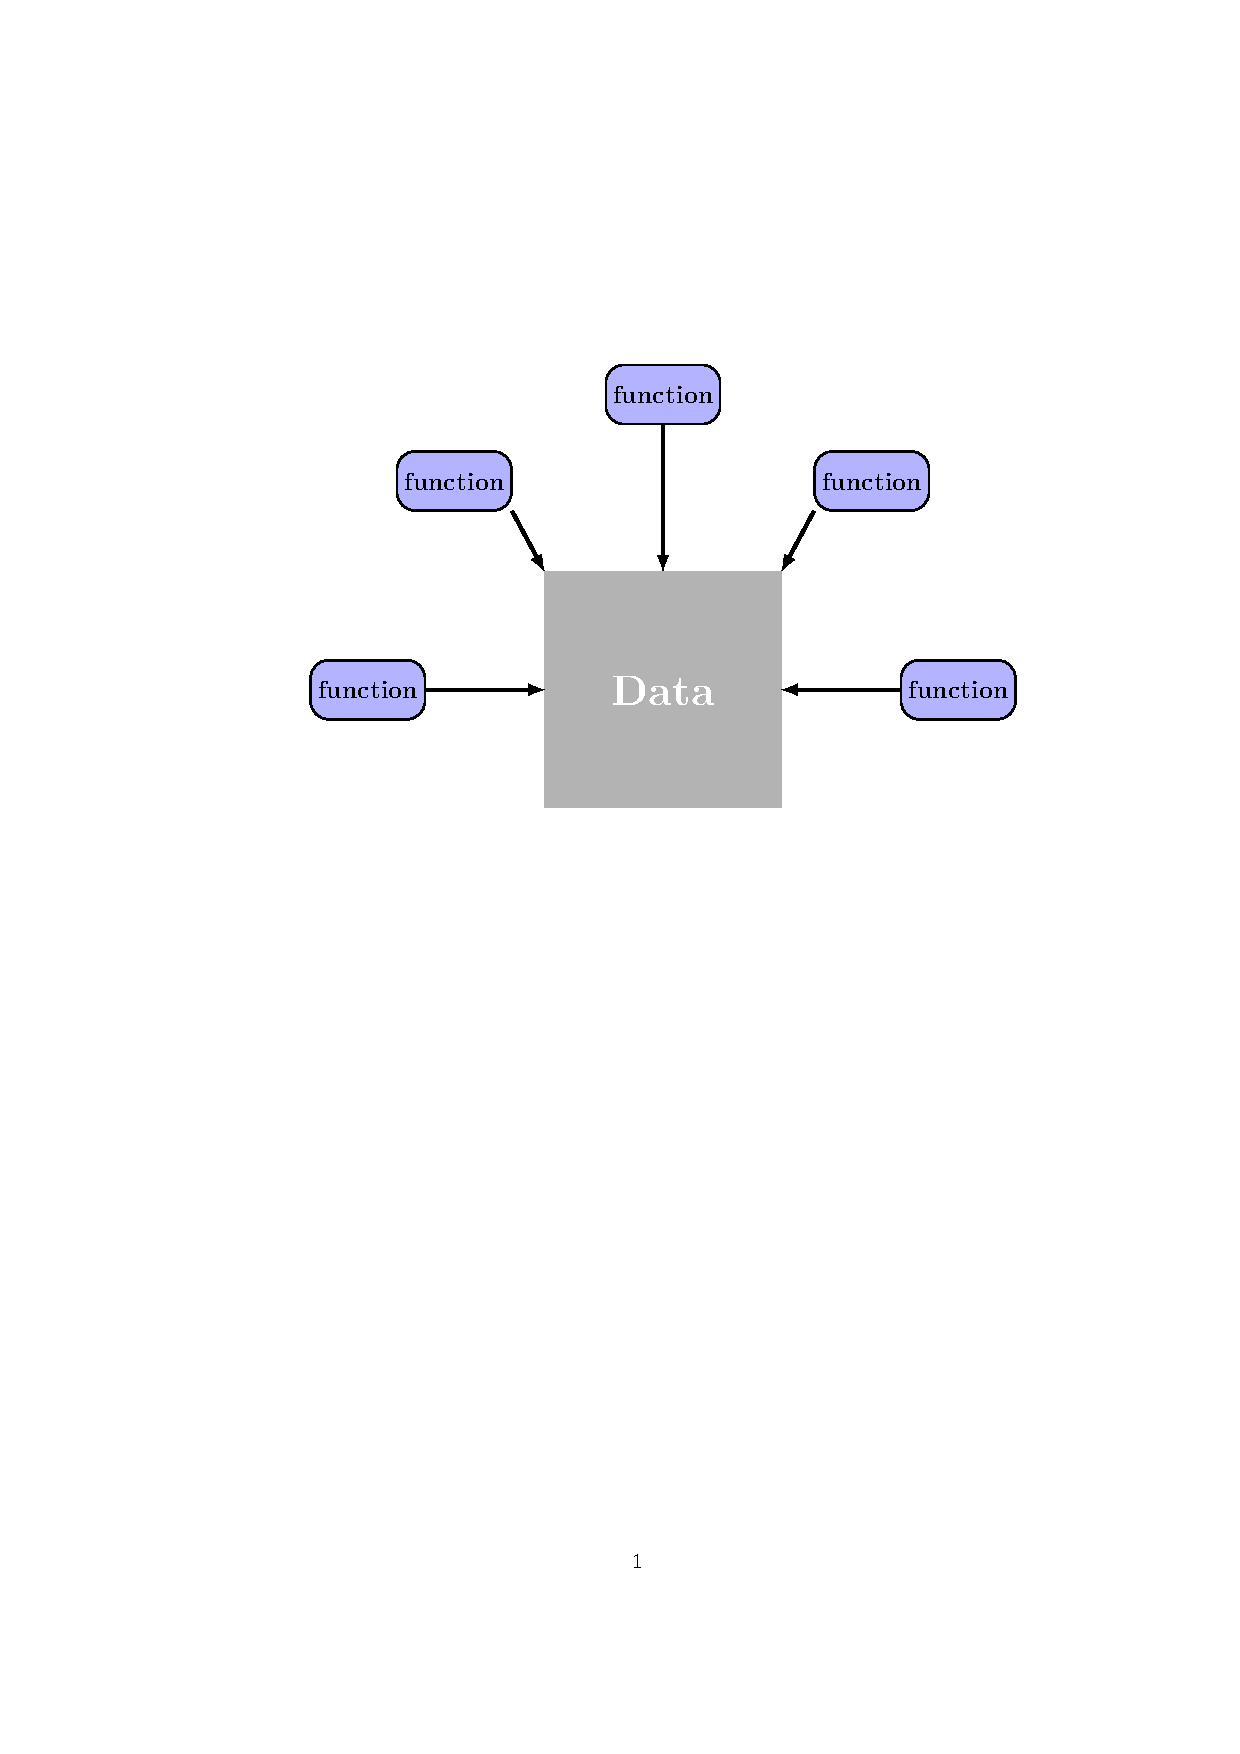
\includegraphics{img/procedural}}
      \end{center}
      \end{block}
   
  \end{column}
\hfill
\pause
  \begin{column}{.49\textwidth}

      \begin{block}{the oo paradigm}
        \begin{center}
        \resizebox{1.\textwidth}{!}{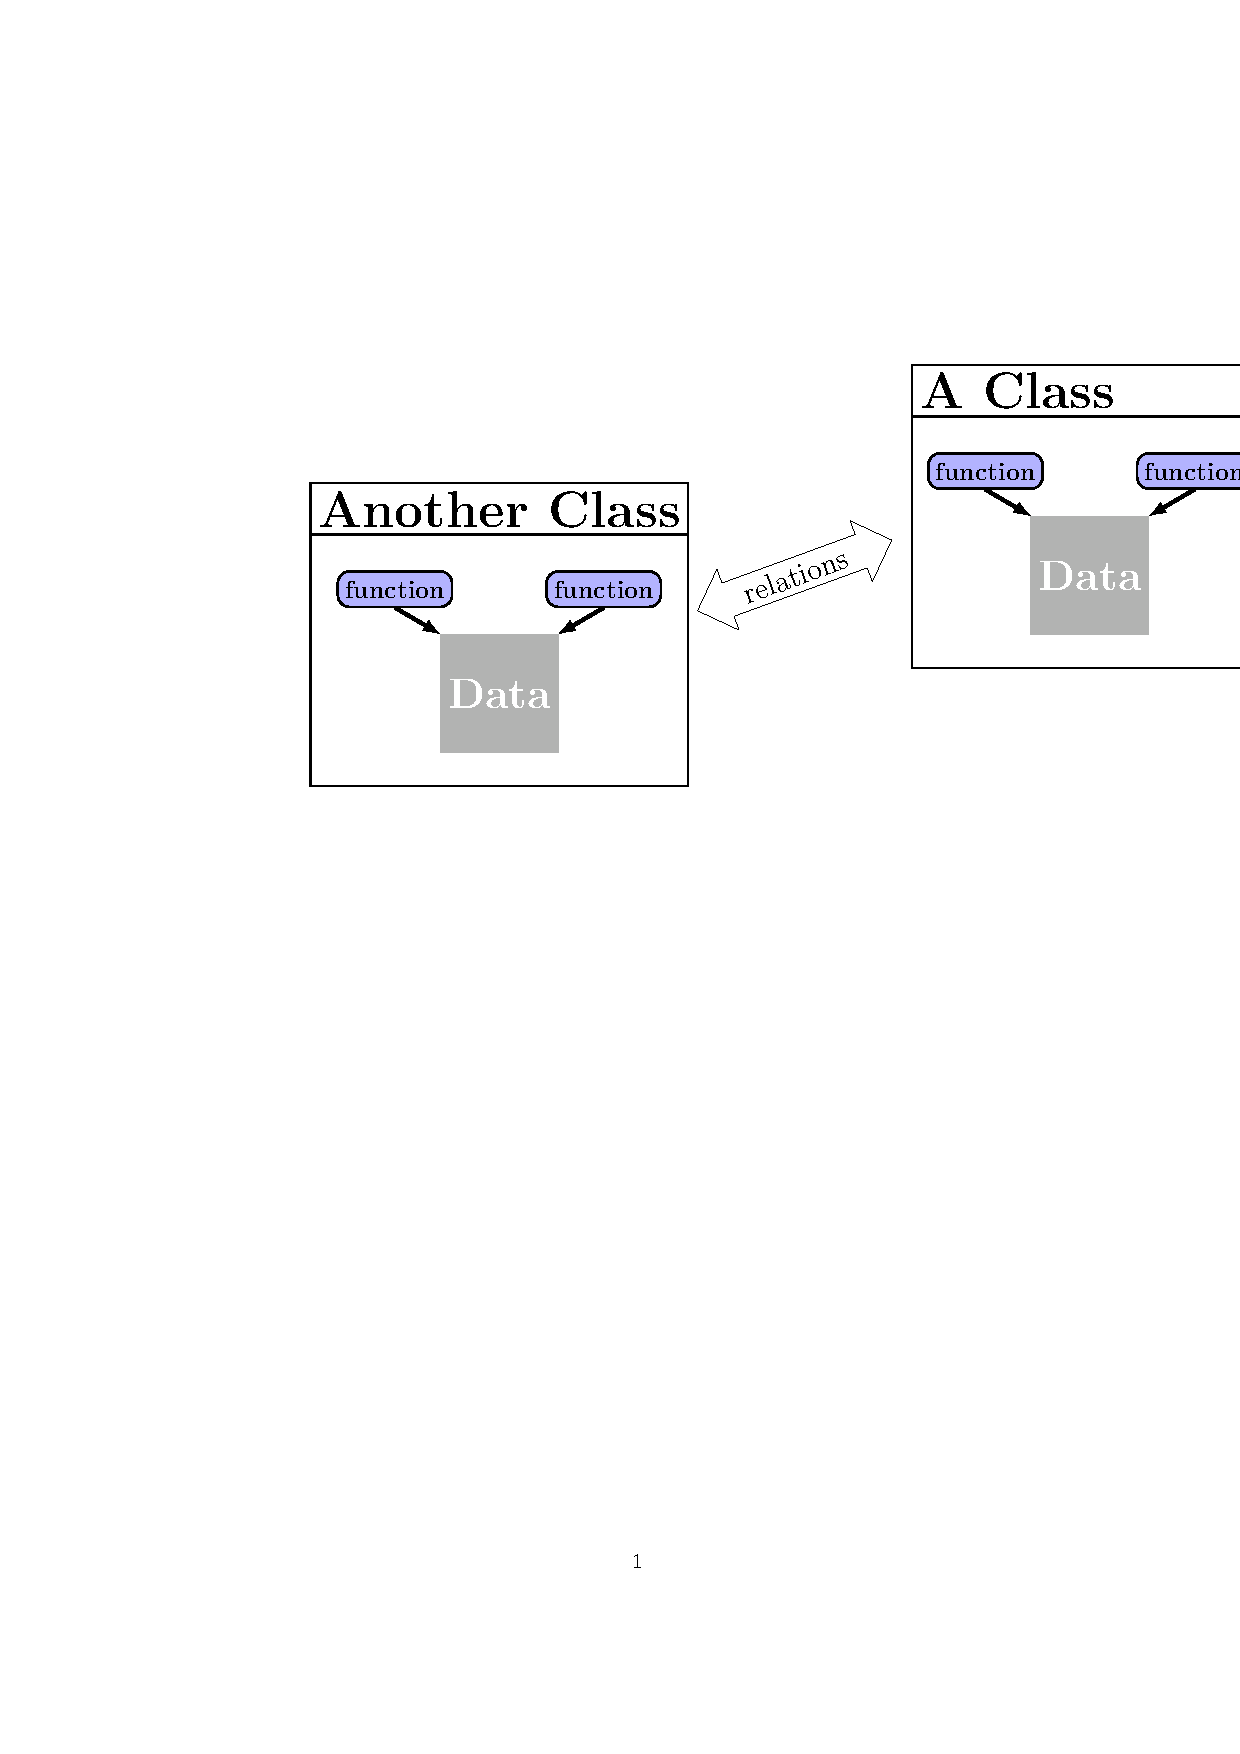
\includegraphics{img/oop}}
        \end{center}
      \end{block}
      
  \end{column}

\end{columns}
\vfill
\begin{columns}[c]
  \begin{column}{.49\textwidth}
    \begin{center}
      \huge
      \alert{Top-Down}
  
    \end{center}
  \end{column}
  \begin{column}{.49\textwidth}
    \begin{center}
      \huge
      \alert{Bottom-Up}
    \end{center}
  \end{column}
\end{columns}
\end{frame}

\subsection[Hep Software]{HEP Programming}
\begin{frame}
\frametitle{Hep Software Sizes}
\begin{block}{A History of Code}
  \begin{center}
    \Large
    \begin{tabular}[h]{l|p{5cm}}
      & lines of code / $\unit[1]{loc}$ \\[12pt]
      JADE & $o(10-100)k$\\[12pt]
      OPAL & $o(100)k$\\[12pt]
      ATLAS & $o(1)M$
    \end{tabular}
  \end{center}
\end{block}
\vfill
\begin{itemize}
\item<2-> experiments size and complexity increases 
\item<3-> experiments analysis software size and complexity increases
\item<4-> \Large \alert{We need tools that deal with this complexity!}
\end{itemize}

\end{frame}

\subsection[OOP in HEP]{Programming Paradigms in HEP}
\begin{frame}
\frametitle{Programming Paradigms in HEP}
\normalsize
\begin{block}{physics is about ...}
  \begin{itemize}
  \item \alert<4->{modelling nature}
  \item objects interact according to laws of nature
    \begin{itemize}
    \item fields, particles, atoms, molecules, solid states, liquids
    \end{itemize}
  \end{itemize}
\end{block}
\vfill
\pause
\begin{block}{object-oriented programming is about ...}
  \begin{itemize}
  \item \alert<4->{objects and interactions}
    \begin{itemize}
    \item a way of thinking about software well adapted to
      physics
    \end{itemize}

  \end{itemize}
\end{block}
\vfill
\pause
\begin{block}{object-oriented analysis and design ...}
  \begin{itemize}
  \item is a software engineering practice
  \item \alert<4->{manages large projects professionally}
  \end{itemize}
\end{block}
\end{frame}

\section{Orthogonality}
\begin{frame}
  \frametitle{Orthogonality}
  \begin{definition}
    A \emph{Responsibility} of a class is defined as \emph{a reason for the class to change}.
  \end{definition}
  %Modem, TSystem examples
  \vfill
  \begin{exampleblock}{Exercise 1}
    \begin{center}
      \Large
      How many responsibilities do classes a) and b) have?
    \end{center}

  \end{exampleblock}
  \vfill
\end{frame}

\begin{frame}
  \frametitle{Single-Responsibility-Principle}
  \begin{theorem}
    A class should only have \textbf{one} reason to change.
  \end{theorem}
\vfill
  \begin{columns}[c]
    \begin{column}{.49\textwidth}
       \begin{block}{before}

         % \begin{center}
         %   %   \resizebox{.85\textwidth}{!}{\includegraphics{img/modem_before}}
         % \end{center}
      %   
       \end{block}
 %     
    \end{column}
    \begin{column}{.49\textwidth}
       \begin{block}{after}
      % \begin{center}
      %   \resizebox{.85\textwidth}{!}{\includegraphics{img/modem_after}}
      % \end{center}
      \end{block}
    \end{column}
  \end{columns}
\end{frame}

\section{Open-Closed}

\section{Liskhov Substitution}

\section{Dependency-Inversion}

\section{Summary}

\section{References}
\scriptsize
\begin{frame}
  \frametitle{References}
  \bibliographystyle{plain} 
  \bibliography{Mar10.ClassDesign}
\end{frame}
\end{document}




